%provide useful commands and default settings
%&pdfLaTeX
% !TEX encoding = UTF-8 Unicode
\documentclass[12pt]{article}
\usepackage[top=1in, bottom=1in, left=1in, right=1in]{geometry}
%\usepackage[cm]{fullpage}
\usepackage[colorlinks=true,linkcolor=NavyBlue,citecolor=Black,urlcolor=Blue]{hyperref}
\usepackage{ifxetex}
\usepackage{url}
\ifxetex
%\usepackage{fontspec}
%\defaultfontfeatures{Mapping=tex-text,Scale=MatchLowercase}
%\setmainfont[Scale=.95]{Times}
\setmainfont[Mapping=tex-text, Scale=2.0]{STIXGeneral}
\else
\usepackage[T1]{fontenc}
\usepackage[utf8]{inputenc}
\usepackage{lmodern}
\fi
\usepackage{textcomp}
\usepackage[square,sort,comma,numbers]{natbib}  % formatting for references
\usepackage{mdframed}
\usepackage{setspace}
%\usepackage{ulem}
%\usepackage{amssymb}
\usepackage{amsmath,amssymb}
\usepackage{graphicx}% Include figure files
\usepackage{longtable} % allow multipage tables
\usepackage{multirow}
\usepackage{psfrag,rotating,multirow,setspace,colordvi}
\usepackage{epstopdf}
\usepackage{dcolumn}% Align table columns on decimal point
\usepackage{bm}% bold math
%\usepackage{subfigure}
%\usepackage{caption}
\usepackage[font=scriptsize,format=plain,labelfont=bf]{caption}
\usepackage{subcaption}
\usepackage{float}
%\usepackage{babel}
\usepackage{makeidx}
%\usepackage[font=footnotesize,format=plain,labelfont=bf,font=doublespacing]{caption}
%\usepackage{overcite}
\usepackage{color}
\usepackage[usenames,dvipsnames,svgnames,table]{xcolor}
\definecolor{color18}{rgb}{0.5,0.5,0.5}

% ==================================================
% Commands and shortcuts that are helpful and specific
% to this document
% ==================================================
\newcommand{\elmer}{\software{Elmer}\,\,}
\newcommand{\foam}{\software{OpenFoam-Extend}\,\,}
\newcommand{\impact}{\software{IMPACT}\,\,}

% ==================================================
% Track changes and commenting packages and commands
% ==================================================
\usepackage{todonotes}
\newcommand{\jek}[1]{\todo[inline,color=purple!40,caption={}]{#1}}
\newcommand{\mdb}[1]{\todo[inline,color=orange!40,caption={}]{#1}}
\newcommand{\mja}[1]{\todo[inline,color=blue!40,caption={}]{#1}}
\newcommand{\mtc}[1]{\todo[inline,color=red!40,caption={}]{#1}}
\newcommand{\sam}[1]{\todo[inline,color=green!40,caption={}]{#1}}
\newcommand{\rxi}[1]{\todo[inline,color=yellow!40,caption={}]{#1}}

%\usepackage[addedmarkup=bf,deletedmarkup=sout]{changes} %Final showing markup
\usepackage[final]{changes} %Final

\definechangesauthor[color=purple]{jek}
\newcommand{\jeka}[1]{\added[id=jek]{#1}}
\newcommand{\jekd}[1]{\deleted[id=jek]{#1}}
\newcommand{\jekr}[2]{\replaced[id=jek]{#1}{#2}}

\definechangesauthor[color=orange]{mdb}
\newcommand{\mdba}[1]{\added[id=mdb]{#1}}
\newcommand{\mdbd}[1]{\deleted[id=mdb]{#1}}
\newcommand{\mdbr}[2]{\replaced[id=mdb]{#1}{#2}}

\definechangesauthor[color=blue]{mja}
\newcommand{\mjaa}[1]{\added[id=mja]{#1}}
\newcommand{\mjad}[1]{\deleted[id=mja]{#1}}
\newcommand{\mjar}[2]{\replaced[id=mja]{#1}{#2}}

\definechangesauthor[color=red]{mtc}
\newcommand{\mtca}[1]{\added[id=mtc]{#1}}
\newcommand{\mtcd}[1]{\deleted[id=mtc]{#1}}
\newcommand{\mtcr}[2]{\replaced[id=mtc]{#1}{#2}}

\definechangesauthor[color=green]{sam}
\newcommand{\sama}[1]{\added[id=sam]{#1}}
\newcommand{\samd}[1]{\deleted[id=sam]{#1}}
\newcommand{\samr}[2]{\replaced[id=sam]{#1}{#2}}

\definechangesauthor[color=yellow]{rib}
\newcommand{\riba}[1]{\added[id=rib]{#1}}
\newcommand{\ribd}[1]{\deleted[id=rib]{#1}}
\newcommand{\ribr}[2]{\replaced[id=rib]{#1}{#2}}
% ==================================================


% ==================================================
% SI units package and special commands
% ==================================================
\usepackage{siunitx}
\newcommand{\SIper}{\SI[per-mode=symbol]}
% ==================================================


% ==================================================
% Special page formatting commands 
% ==================================================

% Shorten or lengthen page by one line (for orphan lines)
\newcommand{\longpage}{\enlargethispage{\baselineskip}}
\newcommand{\shortpage}{\enlargethispage{-\baselineskip}}

% Wrap text to end of line for artificial line break
% (Shift-Enter in Word) for figure placement
\newcommand{\startsquarepar}{%
    \par\begingroup \parfillskip 0pt \relax}
\newcommand{\stopsquarepar}{%
    \par\endgroup}
% ==================================================


\usepackage{wrapfig}
%\usepackage{epstopdf}
%\usepackage[rflt]{floatflt}
\usepackage{fancyhdr}
%\setlength{\headheight}{12pt}
\setlength{\headheight}{25pt}
\setlength{\headsep}{.4in}
\setlength{\textheight}{650pt}
\setlength{\parskip}{5pt}
\setlength{\parindent}{0pt}
%\setlength{\footskip}{.1in}
\renewcommand{\headrulewidth}{.5pt}
\renewcommand{\footrulewidth}{0pt}


\newcommand{\tab}{\hspace{5mm}}

\usepackage{enumerate}

% IR-specific stuff
\usepackage{sectsty}
\allsectionsfont{\bfseries\sffamily}
\newcommand{\irpart}[2]{\part{\textsf{#1}}}
\newcommand{\irpara}[2]{\paragraph{\textsf{#1}}}
\newcommand{\irparanonum}[2]{\paragraph*{\textsf{#1}}}
\newcommand{\irsection}[2]{\section{\textsf{#1}}\label{#2}}
\newcommand{\irsectionnonum}[2]{\section*{\textsf{#1}}\label{#2}}
\newcommand{\irssection}[2]{\subsection{\textsf{#1}}\label{#2}}
\newcommand{\irssectionnonum}[2]{\subsection*{\textsf{#1}}\label{#2}}
\newcommand{\irsssection}[2]{\subsubsection{\textsf{#1}}\label{#2}}
\newcommand{\irsssectionnonum}[2]{\subsubsection*{\textsf{#1}}\label{#2}}
\newcommand{\irtitle}[1]{\title{\bf{\textsf{#1}}}}
\newcommand{\irauthor}[1]{\author{\textsf{#1}}}
\newcommand{\irdate}[1]{\textsf{\date{#1}}}
\newcommand{\irtoday}{\textsf{\today}}
\newcommand{\rocstar}{{\textit{Rocstar}}}
\newcommand{\software}[1]{\textit{#1}}
\newcommand{\irfilename}[1]{\texttt{\textsf{#1}}}
\newcommand{\irwebsite}[1]{\irfilename{\bf #1}}
\newcommand{\commandline}[1]{\texttt{> #1}}
\newcommand{\plusplus}[1]{#1{}\texttt{++}}
\newcommand{\irref}[2]{\hyperref[#2]{#1~\ref{#2}}}
\newcommand{\irrefexp}[3]{\hyperref[#3]{{#1}~{#2}}}
\newcommand{\hilight}[1]{\colorbox{yellow}{#1}}
\def\Dpartial#1#2{ \frac{\partial #1}{\partial #2} }
\def\Dparttwo#1#2{ \frac{\partial^2 #1 }{ \partial #2^2} }
\def\Dpartpart#1#2#3{ \frac{\partial^2 #1 }{ \partial #2 \partial #3} }
\def\Dnorm#1#2{ \frac{d #1 }{ d #2} }
\def\Dnormtwo#1#2{ \frac{d^2 #1 }{ d #2 ^2} }
\def\Dtotal#1#2{ \frac{D #1 }{ D #2} }


\newcommand{\cJ}{\mathcal{J}}
\newcommand{\cI}{\mathcal{I}}
\newcommand{\cM}{\mathcal{M}}
\newcommand{\cP}{\mathcal{P}}
\newcommand{\cN}{\mathcal{N}}
\newcommand{\cC}{\mathcal{C}}
\newcommand{\cG}{\mathcal{G}}

\newcommand{\bx}{\mathbf{x}}
\newcommand{\bn}{\mathbf{n}}

\newcommand{\hh}{{\hat{h}}}
\newcommand{\rh}{{\hat{r}}}

\newcommand{\vvC}{{\Vec{\Vec{c}}}}
\newcommand{\vF}{{\vec{F}}}
%\newcommand{\vf}{{\vec{f}}}
\newcommand{\vb}{{\vec{b}}}
\newcommand{\vq}{{\vec{q}}}
\newcommand{\vR}{{\vec{R}}}
\newcommand{\vqs}{{\vec{q}^{\,*}}}
\newcommand{\vqsT}{{\vec{q}^{\,*T}}}
\newcommand{\vs}{{\vec{s}}}


\newcommand{\bxi}{\boldsymbol{\xi}}


\newcommand{\bbK}{{\mathbb{K}}}
\newcommand{\bbS}{{\mathbb{S}}}
\newcommand{\bbP}{{\mathbb{P}}}
\newcommand{\bbI}{{\mathbb{I}}}
\newcommand{\bbA}{{\mathbb{A}}}
\newcommand{\bbB}{{\mathbb{B}}}
\newcommand{\pOmega}{{\partial\Omega}}

%\providecommand{\e}[1]{\ensuremath{\times 10^{#1}}}

\def\eps{\varepsilon}
\def\bx{\mathbf{x}}
\def\bk{\mathbf{k}}
\def\bkappa{\boldsymbol{\kappa}}


\def\bdash{\hbox{\drawline{4}{.5}\spacce{2}}}
\def\spacce#1{\hskip #1pt}
\def\drawline#1#2{\raise 2.5pt\vbox{\hrule width #1pt height #2pt}}
\def\dashed{\bdash\bdash\bdash\bdash\nobreak\ }
\def\solid{\drawline{24}{.5}\nobreak\ }
\renewcommand{\thefootnote}{\fnsymbol{footnote}}
\renewcommand{\thispagestyle}[1]{} % do nothing

%command to generate the header, put #1 at the right (document title) and #2 centered (release statement)
\newcommand{\irheader}[2]
{
  \pagestyle{fancy}
  \rhead{}
  \rfoot{}
  \chead{}
  %\cfoot{\color{color18}{\thepage{}}}
  \fancyhead[LO,L]{
\includegraphics[width=24pt]{../Figures/IRTriangles.png}\color{color18}\textsf{\space Illinois Rocstar LLC}}
  \fancyhead[RO,R]{\color{color18}{\textsf{#1}}}
  \fancyhead[CO,C]{\color{color18}{\textsf{#2}}}
  \fancyfoot[CO,C]{\color{color18}{\thepage{}}}
}

%Command to generate the copyright page
\newcommand{\ircopyright}[0]
{
  %\clearpage\null
  \vfill
%\pagesytle{empty}
  \begin{minipage}[b]{0.9\textwidth}
  \footnotesize\raggedright
  \setlength{\parskip}{0.5\baselineskip}
  Copyright \copyright\the\year\ Illinois Rocstar LLC\par
  \irwebsite{www.illinoisrocstar.com}
  \end{minipage}
  \vspace*{2\baselineskip}
  \cleardoublepage
}

\newcommand{\ircallout}[3]
{
  \begin{wrapfigure}{#1}{#2\textwidth}
        \vspace{-20pt}
        \centering
        \fbox{\parbox{#2\textwidth}{#3}}
        \vspace{-10pt}
  \end{wrapfigure}
}

\newcommand\todoin[2][]{\todo[inline, caption={2do}, #1]{
\begin{minipage}{\textwidth-4pt}#2\end{minipage}}}

\newcommand{\todoingreen}[1]{\todo[inline, color=green!40]{#1}}            



% add copyright command to /maketitle
\makeatletter
\g@addto@macro{\maketitle}{\ircopyright}
\makeatother

\makeindex
\usepackage{dirtree}

% ******************
%  CALLOUT BOX CONSTRUCT
% ******************
%
%\begin{wrapfigure}{r}{0.3\textwidth}
%        \vspace{-20pt}
%        \centering
%        \fbox{
%             \parbox{0.3\textwidth}{
%                  This is a test of a callout box. 
%                  It has several lines and even a paragraph.
%
%                  See here for the new paragraph. This paragraph
%                  no longer has a bulleted list.
%             }                      
%        }
%        \vspace{-10pt}
%\end{wrapfigure}


%------------------------------------------------------------------
% Includeed Packages
%------------------------------------------------------------------
\usepackage{enumitem}
\usepackage{fancybox}
\usepackage{threeparttable}
\usepackage{multicol}
\usepackage[export]{adjustbox}

\usepackage{titlesec}
\titlespacing*{\section}{0pt}{2.5ex plus 1 ex minus .5ex}{1.5ex plus .75ex minus .5 ex}
\titlespacing*{\subsection}{0pt}{2ex plus .5ex minus .25ex}{1ex plus .5ex minus .25ex}
\titlespacing*{\subsubsection}{0pt}{1.5ex plus .5ex minus .25ex}{.75ex plus .5ex minus .25ex}
\titlespacing*{\paragraph}{0pt}{1ex plus .25ex minus .25ex}{.5ex plus .25ex minus .25ex}

%------------------------------------------------------------------
% New Commands: Programs
%------------------------------------------------------------------
\newcommand{\impact}{\software{IMPACT}}
\newcommand{\IMPACT}{\software{IMPACT}}
\newcommand{\icofoam}{\software{IcoFoam}}
\newcommand{\openfoam}{\software{OpenFoam}}
\newcommand{\openfoamex}{\software{OpenFoam Extend}}

\def\cpp{C{}\texttt{++}}

\newcommand{\wbs}[1]{\textcolor{MidnightBlue}{\textsf{WBS\# #1}}}
\newcommand{\subcap}[1]{{\footnotesize #1}}
\newcommand{\mybox}[1]{\doublebox{\parbox{0.97\textwidth}{{#1}}}}
\newcommand{\term}[1]{{\textbf{\textsf{#1}}}}
\newcommand{\snoteTe}[1]{{\textcolor{red}{\textbf{#1}}}}
\renewcommand{\vec}[1]{\mathbf{#1}}

\newcommand{\vv}{V\&V}
\newcommand{\x}[1]{$#1\times$}
\newcommand{\percent}[1]{#1\%}
\newcommand{\siper}{\SI[per-mode=symbol]}
\newcommand{\g}{\gram}
\newcommand{\ms}{\milli\second}
\newcommand{\m}{\meter}
\newcommand{\cm}{\centi\meter}
\newcommand{\mm}{\milli\meter}
\newcommand{\um}{\micro\meter}
\newcommand{\nm}{\nano\meter}
\newcommand{\kpa}{\kilo\pascal}
\newcommand{\mpa}{\mega\pascal}
\DeclareSIUnit\pixel{pixel}
\DeclareSIUnit\ppm{ppm}
\DeclareSIUnit\amu{amu}
\DeclareSIUnit\in{in}
\DeclareSIUnit\psi{psi}
\DeclareSIUnit\psia{psia}
\DeclareSIUnit\psig{psig}
\newcommand{\mpix}{\mega\pixel}

\newcommand{\chem}[1]{\mathrm{#1}}

%------------------------------------------------------------------
% New Commands: Contract information
%------------------------------------------------------------------
\newcommand{\cnum}{NNX14CA36P}
\newcommand{\connum}{Contract No. \cnum}
\newcommand{\conname}{Integrated Computational System for Electrochemical Device Design and Simulation}
\newcommand{\rptname}{Quarterly (interim) demonstration report}

%------------------------------------------------------------------
%  These two lines will number figures and tables as #1.#2, where #1
%  number of chapter and #2 is the figure or table number within the chapter
%------------------------------------------------------------------
\renewcommand{\thefigure}{\thesection.\arabic{figure}}
\renewcommand{\thetable}{\thesection.\arabic{table}}
\renewcommand{\theequation}{\thesection.\arabic{equation}}
\renewcommand{\thefootnote}{\fnsymbol{footnote}}

%==================================================================
% Document build
%==================================================================

\begin{document}

%Information for the Title page
\pagestyle{fancy}

\begin{figure}
  \centering
  
\includegraphics[height=3.in]{../Figures/IR_Logo.png}
\end{figure}
%-----------------------------------------------
\irtitle{\impact\, Module for \icofoam}
\irauthor{Illinois Rocstar LLC}
\date{\textsf{\today}}

\pagestyle{empty}
\maketitle

\setcounter{secnumdepth}{5}
\setcounter{tocdepth}{4}


\irheader{\connum}{}
\newpage
\thispagestyle{empty}

\newpage
\renewcommand{\contentsname}{Table of Contents}
\tableofcontents

%\newpage
\listoffigures
\listoftables
\newpage
\pagenumbering{arabic}
\setcounter{page}{1}

\irsection{OpenFoam}{OpenFoam}

In order to build a module for \icofoam\, it is necessary to first download and build \openfoam\, and specifically for this case \openfoamex\, (\openfoam\, and \openfoamex\, will be used interchangeably within this document).  Information for downloading this software can be found at \url{http://www.extend-project.de/}.

\textbf{Note:} The same \software{mpicc}, \software{mpicxx}, and/or \software{mpif90} must be used when compiling \software{IMPACT}, \openfoam, and the module driver. 

\jek{Is the above correct, Mike C.? I couldn't remember if I had set those variables before compiling \openfoam\, but I assume I did}

For builds outside of Illinois Rocstar make note of the compiler used to build \openfoam\, and then follow the build instructions for \openfoam\, found online or in the documentation. If you are working within Illinois Rocstar then load the \irfilename{openmpi-x86\_64} module and set the environment variables \irfilename{CC}, \irfilename{CXX}, and \irfilename{FC} to \irfilename{mpicc}, \irfilename{mpicxx}, and \irfilename{mpif90} respectively. Then, source the appropriate file (\irfilename{cshrc} when using \software{C Shell} or \irfilename{bashrc} when using \software{Bash}) found in the \irfilename{etc} directory under the main \software{OpenFoam} source directory by entering one of the following commands

\commandline{source etc/cshrc} 

or
 
\commandline{source etc/bshrc}

from the main \openfoam\, source directory. Finally, run

\commandline{wmake/wmake all} 

from the main \openfoam\, source directory. There may be additional changes that must be made to the \irfilename{wmake} files in order to get \openfoam\, to properly compile within your specific environment setup. 

After \openfoam\, is built, ensure that the \irfilename{icofoam} executable has been created. If you have sourced one of the files for \openfoam\, as mentioned above you may check that the \irfilename{icofoam} executable exists by running 

\commandline{which icofoam}

and ensuring that the \irfilename{icofoam} command returned is within the path of the \openfoam\, source files you have been building (\openfoam\, builds in-source).

Within Illinois Rocstar, a test case exists for \icofoam\, from \openfoamex. The documentation for this test case can be found in Section 9.2.2 of the \irfilename{Uniphysics Validation for Development of Multiphysics Coupling in MP-Infra} document located internally in the Illinois Rocstar source repository under \irfilename{/MPInfra/data/documentation/validation\_uniphysics/Tex}. After ensuring that the test run works, the next steps toward building a module can be taken.

\irsection{\software{IMPACT}}{IMPACT}

The Illinois Rocstar software \IMPACT\, is required for integrating the \icofoam\, module. For an external user the \IMPACT\, software may be downloaded from \url{http://sourceforge.net/p/openmultiphys/wiki/Consortium\%20for\%20Open\%20Multiphysics/}. For an internal user, \impact\, is located in the repository under \irfilename{IMPACT/trunk}. Follow the build instructions from the User's Guide. Note that internal users may not need to build \impact\, but instead simply load the \impact\, module provided to their machine. 

Ensure that the locations of the \impact\, \irfilename{include} and \irfilename{lib} directories are known since they will be needed in \irref{Section}{ModuleFiles}. If you use \texttt{make install} when installing \impact\, these directories should both be located under the install directory. Otherwise, they should be located in the main source directory and the main build directory for \impact\, respectively.
\irsection{Obtaining, placing, and editing the module files}{ModuleFiles}

For a user internal to Illinois Rocstar the files necessary for building a module for \icofoam\, within \openfoamex\, can be found in the source repository under \irfilename{/MPInfra/Third\_Party\_ Modules/OFTest/icoFoam/trunk/}. For an external user these files may be found on the open multiphysics website (to come). The files will contain the appropriate directory structure for building the driver. However, the files used with \openfoam\, to create a module library must be placed in the appropriate locations within the \openfoam\, source files in order for them to build. These files are located under the \irfilename{native} directory of the module main source directory. The locations for placing these files will be given, but it should be noted that these are specific for \openfoamex\, \software{3.1}. In the case of another version of \openfoamex\, it may be necessary to place these files in different locations. If you are using a different version of \openfoamex\,, it is suggested that you locate the source file \irfilename{icoFoam.C} and then place the module files in a manner with a similar structure to that shown here. 

All paths below are shown from within the \openfoamex\, main source directory.

\begin{itemize}
\item The main source file \irfilename{icoFoam.C} should be located under \newline \irfilename{applications/solvers/incompressible/icoFoam/}.
\item Place \irfilename{icoFoamHeader.H} and \irfilename{icoFoamModule.C} in \newline \irfilename{applications/solvers/incompressible/icoFoam/}.
\item Replace the \irfilename{files} and \irfilename{options} files located under \newline \irfilename{applications/solvers/incompressible/icoFoam/Make} with the \irfilename{files} and \irfilename{options} files provided with the module. (The \irfilename{options} file will require editing.)
\item Place the \irfilename{Allwmake} file in \irfilename{applications/solvers/incompressible/}.
\end{itemize}

It is necessary to edit the \irfilename{options} file in the \irfilename{Make} directory as mentioned above. The \irfilename{options} file should appear as shown below

\begin{mdframed}[]
\begin{verbatim}
EXE_INC = \
    -I$(LIB_SRC)/finiteVolume/lnInclude \
    -I/path/to/IMPACT/install/include

LIB_LIBS = \
    -lfiniteVolume \
    -llduSolvers \
    -L/path/to/IMPACT/install/lib \
    -lSITCOM
\end{verbatim}
\end{mdframed}

Edit the locations that say ``\texttt{path/to/IMPACT/install/}'' to be the actual path to your installation of \software{IMPACT}. Again, note that if you did not do \irfilename{make install} when compiling and building \impact\, the path to the include directory should be the source directory for \impact, and the path to the \irfilename{lib} directory should be the build directory for \impact.

The module files are now in place and have been edited, so the module library can be built.


\irsection{Building the module library and driver}{BuildModule}

In order to build the \elmer module library, simply repeat the build steps taken when building \elmer for the first time (see \irref{Section}{elmer}). However, now \elmer will require the \software{IMPACT} libraries for the build since the new source files added for the module require them. If you installed \software{IMPACT} in a non-standard location you will need to specify the location of the \software{IMPACT} libraries for \software{CMake}. After the  building completes, ensure that the \elmer module library built; it is entitled \irfilename{libSolverModule.so}. It should be located under the \irfilename{lib} directory of the \elmer installation (be sure to run \texttt{make install}).

If the library built successfully, the driver for the module may now be built and linked to both \impact\, and the module library. It is recommended that the driver source and build files be kept in separate directories from one another and from \elmer\!\!. The build steps are as follows:

\begin{itemize}
\item Create a build directory for the driver. 
\newline Example:
\newline \commandline{mkdir /home/user/ElmerModuleBuild}
\item Change directories to the build directory. 
\newline Example:
\newline \commandline{cd /home/user/ElmerModuleBuild}
\item Run \software{CMake} on the module driver source directory with the \texttt{CMAKE\_PREFIX\_PATH} set to both the \IMPACT\, install location (or locations of the \impact\, \irfilename{bin} and \irfilename{lib} directories) and the directory containing the \elmer installation (or the location of the \elmer \irfilename{lib} directory). 
\newline Example:
\newline \commandline{cmake -DCMAKE\_PREFIX\_PATH=/home/user/IMPACT-install$\backslash$; \newline /home/user/elmer-install /home/user/ElmerModule} 
\newline (\textbf{Note} that there is no space between $\backslash$\texttt{;} and \texttt{/home/user/elmer-install}. The new line shown above is used only for visual clarity.)
\item Run \texttt{make} and, if desired, \texttt{make install}.
\end{itemize}

\textbf{Note} that \elmer may install more libraries in the installation directory under \irfilename{share/elmersolver/lib/}. You can either create a soft link to these libraries in the \irfilename{elmer-install/lib} or you can include this directory in the \texttt{CMAKE\_PREFIX\_PATH} by appending it after another $\backslash$; in the \texttt{cmake} command shown above.

Once the build process has finished ensure that the module driver built by checking the \irfilename{bin} directory within the module driver build directory for \irfilename{SolverModuleDriver.}

\irsection{Runing and testing the \icofoam\, module}{RunModule}

Now that the library and driver for the module have been built, run the driver executable in the same manner in which \elmer was run in the example problem discussed in Section 4.3 and 4.4 of the \irfilename{Uniphysics Validation for Development of Multiphysics Coupling in MP-Infra} document (mentioned in \irref{Section}{elmer}). \textbf{Note:} Remember to double check your environment variables. Ensure that the module driver achieves the same results as using the initial \texttt{Elmer} executable. \irref{Figure}{fig:elasticBeam} shows the results of the simulation.
 
\begin{figure}[H]    
\centering
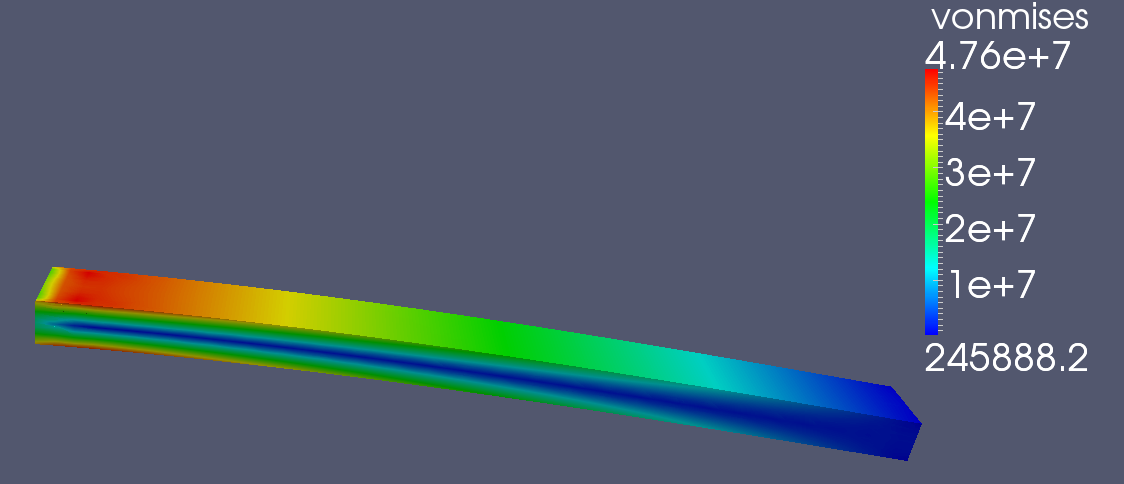
\includegraphics[width=0.85\textwidth]{../Figures/elasticbeam.png}
\caption{Results of elastic beam example run with \software{Elmer IMPACT} module}.
\label{fig:elasticBeam}
\end{figure}


%\newpage

\end{document}
